\documentclass{article}

% if you need to pass options to natbib, use, e.g.:
%     \PassOptionsToPackage{numbers, compress}{natbib}
% before loading neurips_2020

% ready for submission
%\usepackage{neurips_2020}

% to compile a preprint version, e.g., for submission to arXiv, add add the
% [preprint] option:
    % \usepackage[preprint]{neurips_2020}

% to compile a camera-ready version, add the [final] option, e.g.:
%     \usepackage[final]{neurips_2020}

% to avoid loading the natbib package, add option nonatbib:
\usepackage{neurips_2020}
\usepackage{inputenc} % allow utf-8 input
\usepackage[T1]{fontenc}    % use 8-bit T1 fonts
\usepackage{hyperref}       % hyperlinks
\usepackage{url}            % simple URL typesetting
\usepackage{booktabs}       % professional-quality tables
\usepackage{graphicx, float}
\usepackage{amsfonts}       % blackboard math symbols
\usepackage{nicefrac}       % compact symbols for 1/2, etc.
\usepackage{microtype}      % microtypography

\title{Data and Programming for Public Policy II: \\ Final Project Report}


\begin{document}

\maketitle


\section{Introduction}

This project explores tweets that ``hashtagged" Donald Trump and those ``hashtagged" Joe Biden during the 2020 US Presidential Election. I analyzed the setiments of those tweets, estimated the effect of campaign events on candidate's presence on Twitter, and visualized the geographical distribution of popular tweets along with their contents.   

\section{Data}

I used three datasets for tweets and campaign event history. 
\begin{itemize}
	\item Tweets hashtagged Donal Trump
	
	File name: \verb|hashtag_donaldtrump.csv|
	
	\item Tweets hastagging Joe Biden
	
	File name: \verb|hashtag_joebiden.csv|
	
	\item 2020 Presidential Candidate General Election Events Tracker 
	
	File name: \verb|2020 Presidential Candidate General Election Events Tracker(maintained by|
	\verb| FairVote, Nov Version).xlsx|
\end{itemize}
In the project report, I refer to the first two datasets as tweets, and the third as campagin events.

Tweets were collected by Kaggle user \href{https://www.kaggle.com/manchunhui/us-election-2020-tweets}{Manch Hui}. The campaign events were maintained by \href{https://docs.google.com/spreadsheets/d/1oR_x3wGpFi1wO2V0BNMV529s_V-AgGH7tKd66DD7rrM/edit#gid=2025398596}{FairVote}
\section{Research Questions}

I intended to explore three questions: 
\begin{enumerate}
	\item Overall, whether the tweets hashtagged Trump and those hashtagged Biden expressed different sentiments?
	\item Does campaign events promote candidates' presence on Twitter?
	\item What did the most popular tweets say about the two candidates, and how those tweets distributed geographically?
\end{enumerate}


\section{Approach and Coding}

\subsection{Data Wrangling}
	
	Tweets data were in two separate \verb|.csv| files. I merged them into one tidy dataset to perform event study, and extracted tweets into \verb|.txt| files for sentiment analysis.  To remove tweets from potential twitter ``bots", I dropped tweets from users joining later than 2020-01-01 AND with no more than 5 followers.
	
	Campagin events were organized in a wide format. One row of observation corresponded to two events: one is by Biden/Harris, the other by Trump/Pence. I cleaned the campaign events into a tidy data format. 
	
	The script for this step is \verb|step1_data_wrangling.R|.
	
\subsection{Sentiment Analysis}
	
	I tokenized and stemmed the tweets that hashtagged either Trump or Biden. \footnote{For simplicity, I did not extract or analyze tweets that hashtagged both candidates.} I used Bing sentiment lexicon and NRC emotion lexicon. 
	
	The script for this step is \verb|step2_text_analysis.R|.
	
	\paragraph{Results of sentiment analysis} Overall, compared with the tweets that hashtagged Trump, those hashtagged Biden expressed more positive sentiments, such as ``Anticipation", ``Joy", and ``Trust". I presented the results in figure \ref{fig:0}

\subsection{Event Study}
	
	My second research question intends to explore if campaign events promote candidates' presence on Twitter. In a simple DID setting, where treatment\footnote{In our context, the treatment is candidates' campaign visits.} starts at the same time for all
	treated units\footnote{I used states as units.}, it is straightforward to investigate the pre-trend. But candidates visit different states at different times. To investigate the pre-trend, we need to aggregate over multiple campaign visits and define event time $k$ in the following way:
	
	Suppose a candidate visited state $i$ at date $t_i^*$. Let the date $t$ be given, we define the event time $k = t - t_i^*$. 
	
	I define the window for each event to be 2. That is, we will consider the tweets two days prior to the campaign visit, and two days after the visit. This is meant to obtain a balanced panel and minimize the overlap between different events.  

To estimate the average effect of campaign visits on the number of tweets hashtagged the candidates from the visited state, I fitted the model
\begin{equation} \label{eqn:1}
	tweets_{it}=\alpha_{i} +\sum_{k=-2}^{2} \phi_{k} D_{i t}^{k}+u_{i t}
\end{equation}
where $tweets_{it}$ is the number of tweets hashtagged the visiting candidate from a state $i$ on a date $t$, $\alpha_i$ is the state fixed effects so we can preserve the daily variation in the coefficients, $\phi_k$ is the average treatment effect on the treated states, $D_{it}^k$ is the dummy variable for event time $k$ in state $i$ on date $t$. 

To simplify the event study analysis, I removed those VP candidates' visits because I didn't collect tweets that specifically hashtagged Harris or Pence. I also imposed the homogeneous treatment effects across all visited states, and separately fitted the model for those tweets hashtagged Trump and those hashtaging Biden. 

The script for this step is \verb|step3_analysis.R|.

\paragraph{Effect of Campaign Events on Twitter Presence}
The number of tweets hashtagged Trump changes volatilely with his campaign event time. From the figure \ref{fig:1}, the number of tweets hashtagged Trump increased a lot on the days of his campaign visits. While the number of tweets hashtagged Biden are not very correlated with his event time -- the number of tweets hashtagged Biden even dropped on the days of his campaign visits. 

Our analysis concludes that campaign events do not have significant impact on candidates' presence on twitter: most of the effects shown in figure \ref{fig:1} and figure \ref{fig:2} are null effects.

\subsection{Interactive Plot}

I built an interactive map showing the contents of tweets hashtagged Biden or Trump in the election year, the ``like" counts, and the locations. 

The script for this step is \verb|step4_interactive_plot/app.R|. The published web application is \href{https://celia-zhu.shinyapps.io/2020_election_tweets_map/}{here}.

\section{Discussion}

\subsection{Selection Bias}
Twitter users are self-selected. According to \href{https://www.pewresearch.org/internet/2019/04/24/sizing-up-twitter-users/}{an analysis by Pew Research}, Twitter users are younger, more educated, and more likely to be Democrats than general public. 

The tweets in my sample expressed more negative sentiments towards Trump. But this does not represent the general public's view. For the same reason, the tweets sentiment analysis does not enable us to predict the election results. 

\subsection{Future Research}
I'm interested in using network analysis to find out the key Twitter influencers in the 2020 Presidential Election, analyze the sentiments of their tweets related to the election, and visualize their geographic distribution and the network centered around them. 

\pagebreak
\section{Figures}
	
\begin{figure}[h] 
	\begin{center}
		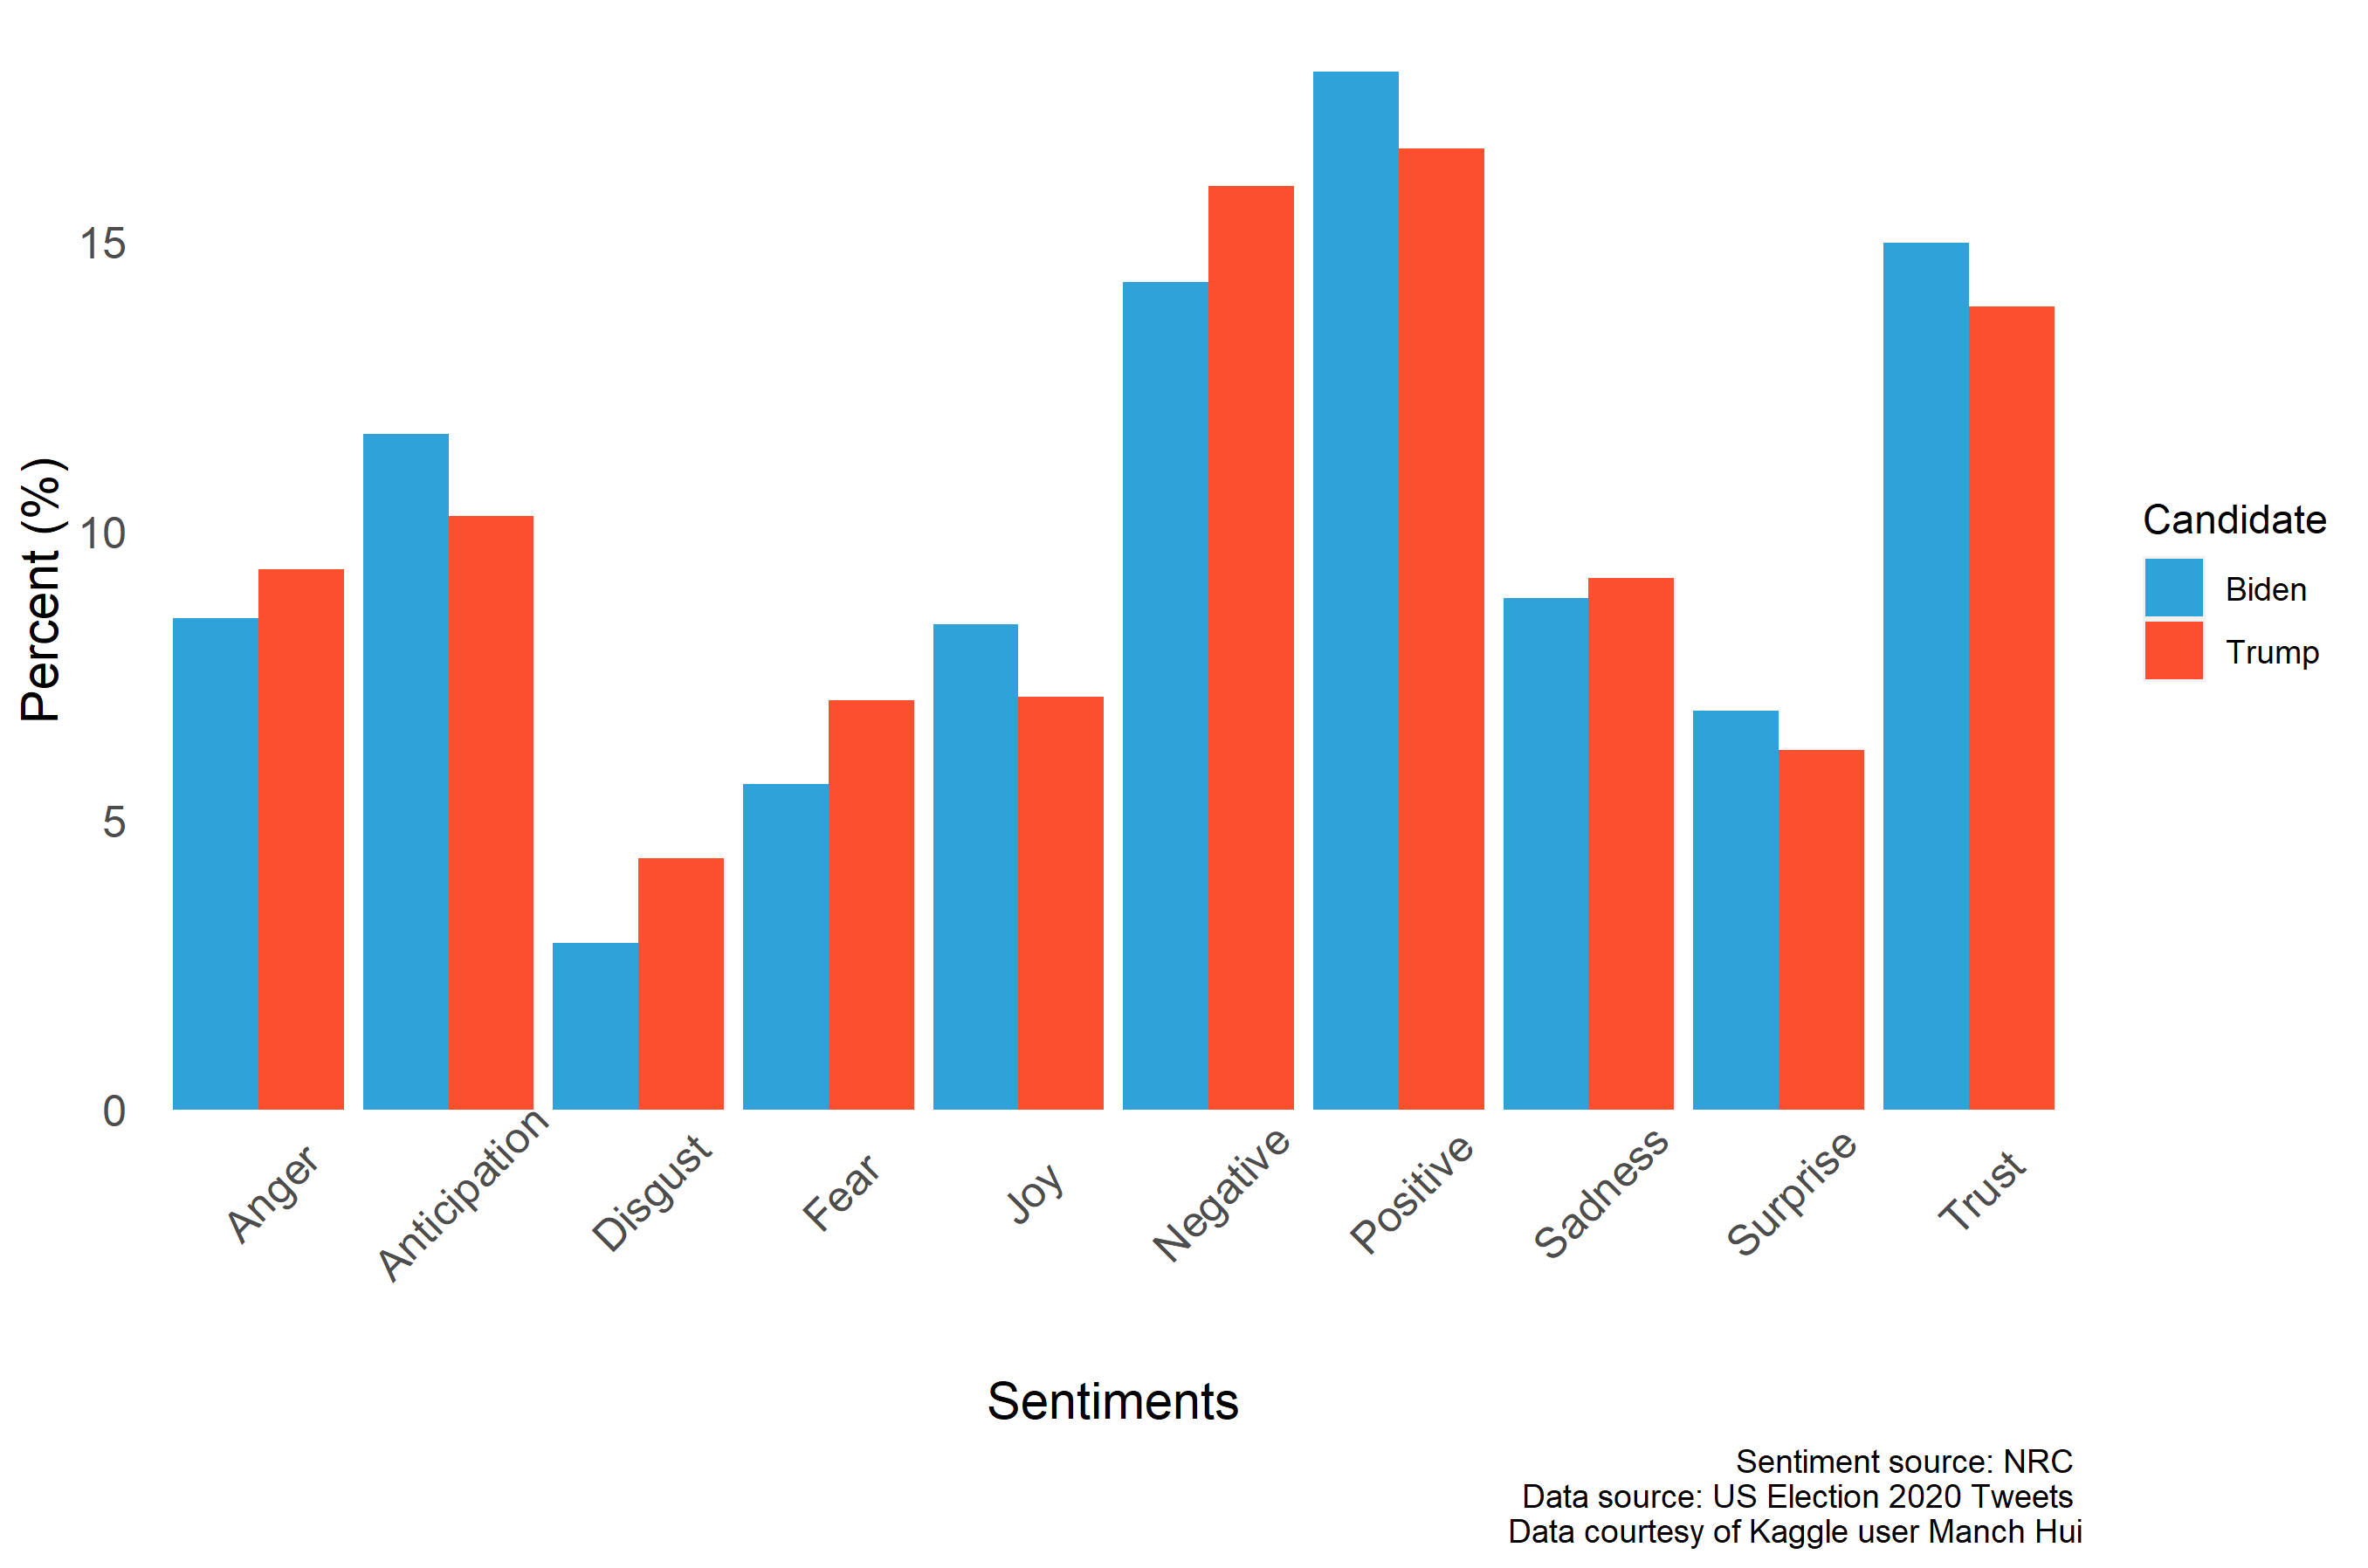
\includegraphics[width = 0.8\textwidth]{C:/Users/Zhuxl/Box/projects/ra_code_sample/election_tweets/output/figures/nrc.png}
		\caption{Sentiment analysis using NRC emotion lexicon} \label{fig:0}
	\end{center}
\end{figure}

\begin{figure}[h]
	\begin{center}		
		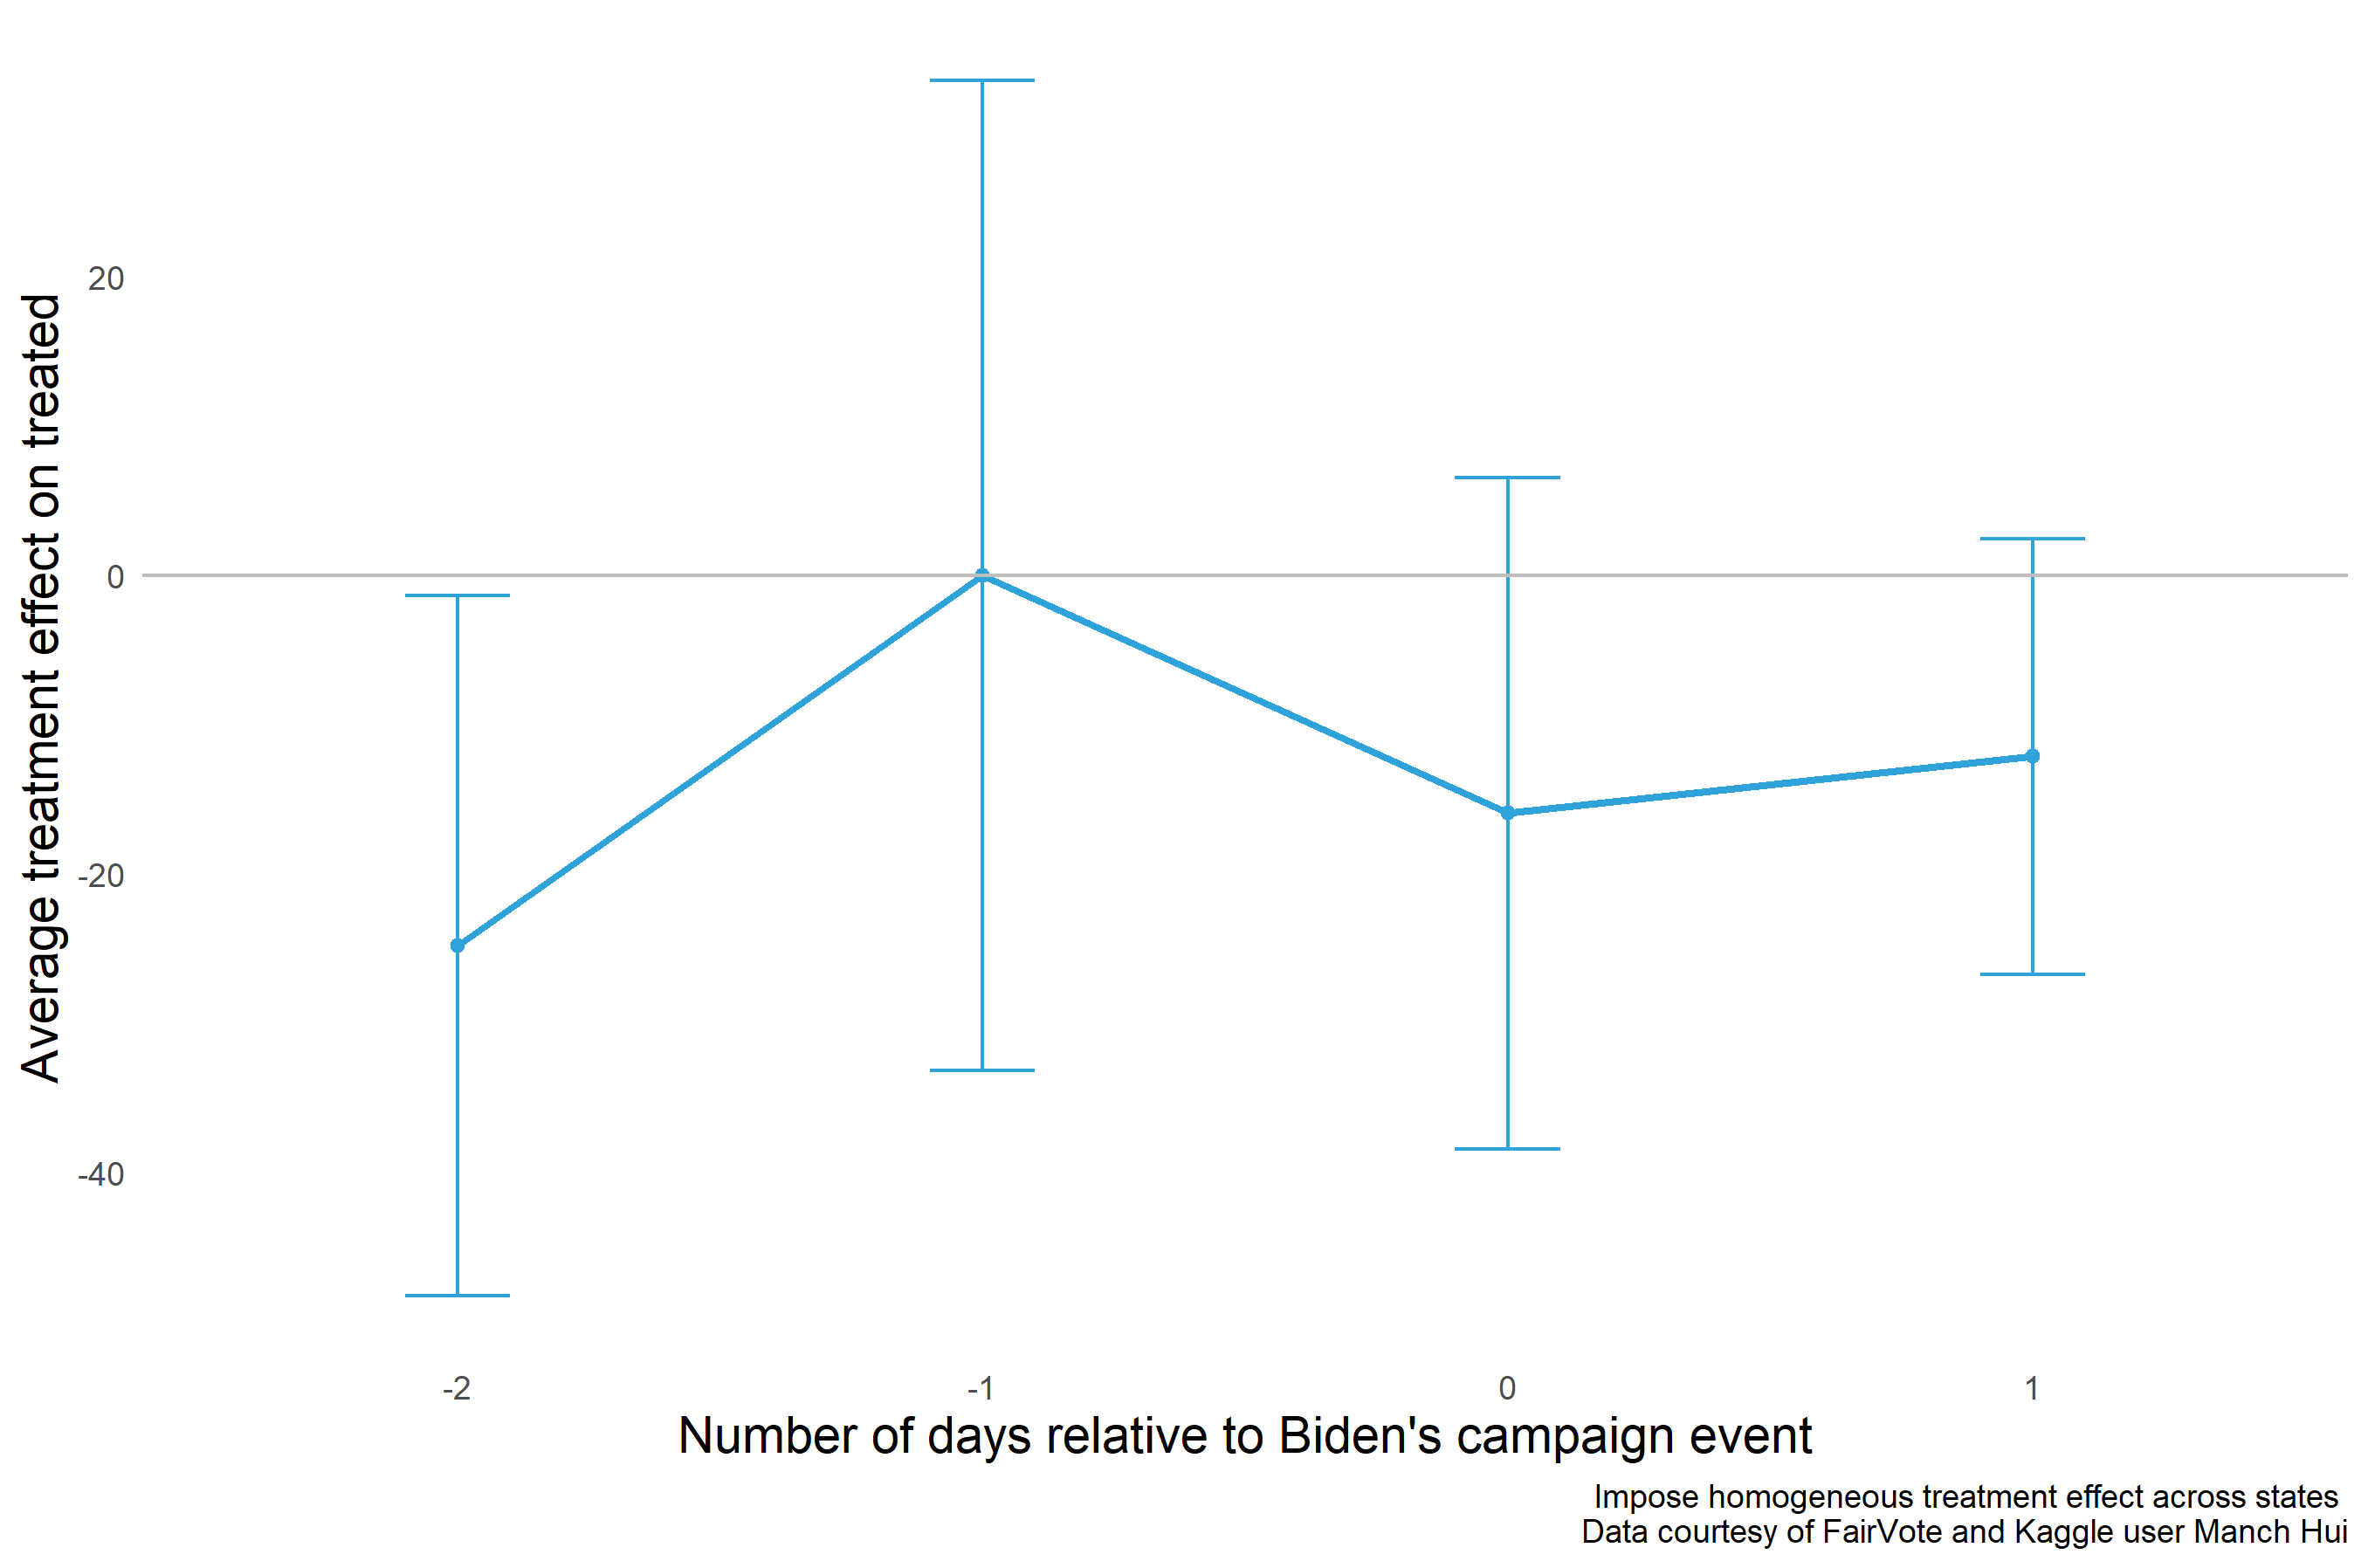
\includegraphics[width = 0.8 \textwidth]{C:/Users/Zhuxl/Box/projects/ra_code_sample/election_tweets/output/figures/event_study_reg_plot_biden.png}
		\caption{Average treatment effect over event time for Biden's twitter presence (impose homogeneous treatment effect across states)}\label{fig:1}
	\end{center}
\end{figure}

\begin{figure}[h]
	\begin{center}
		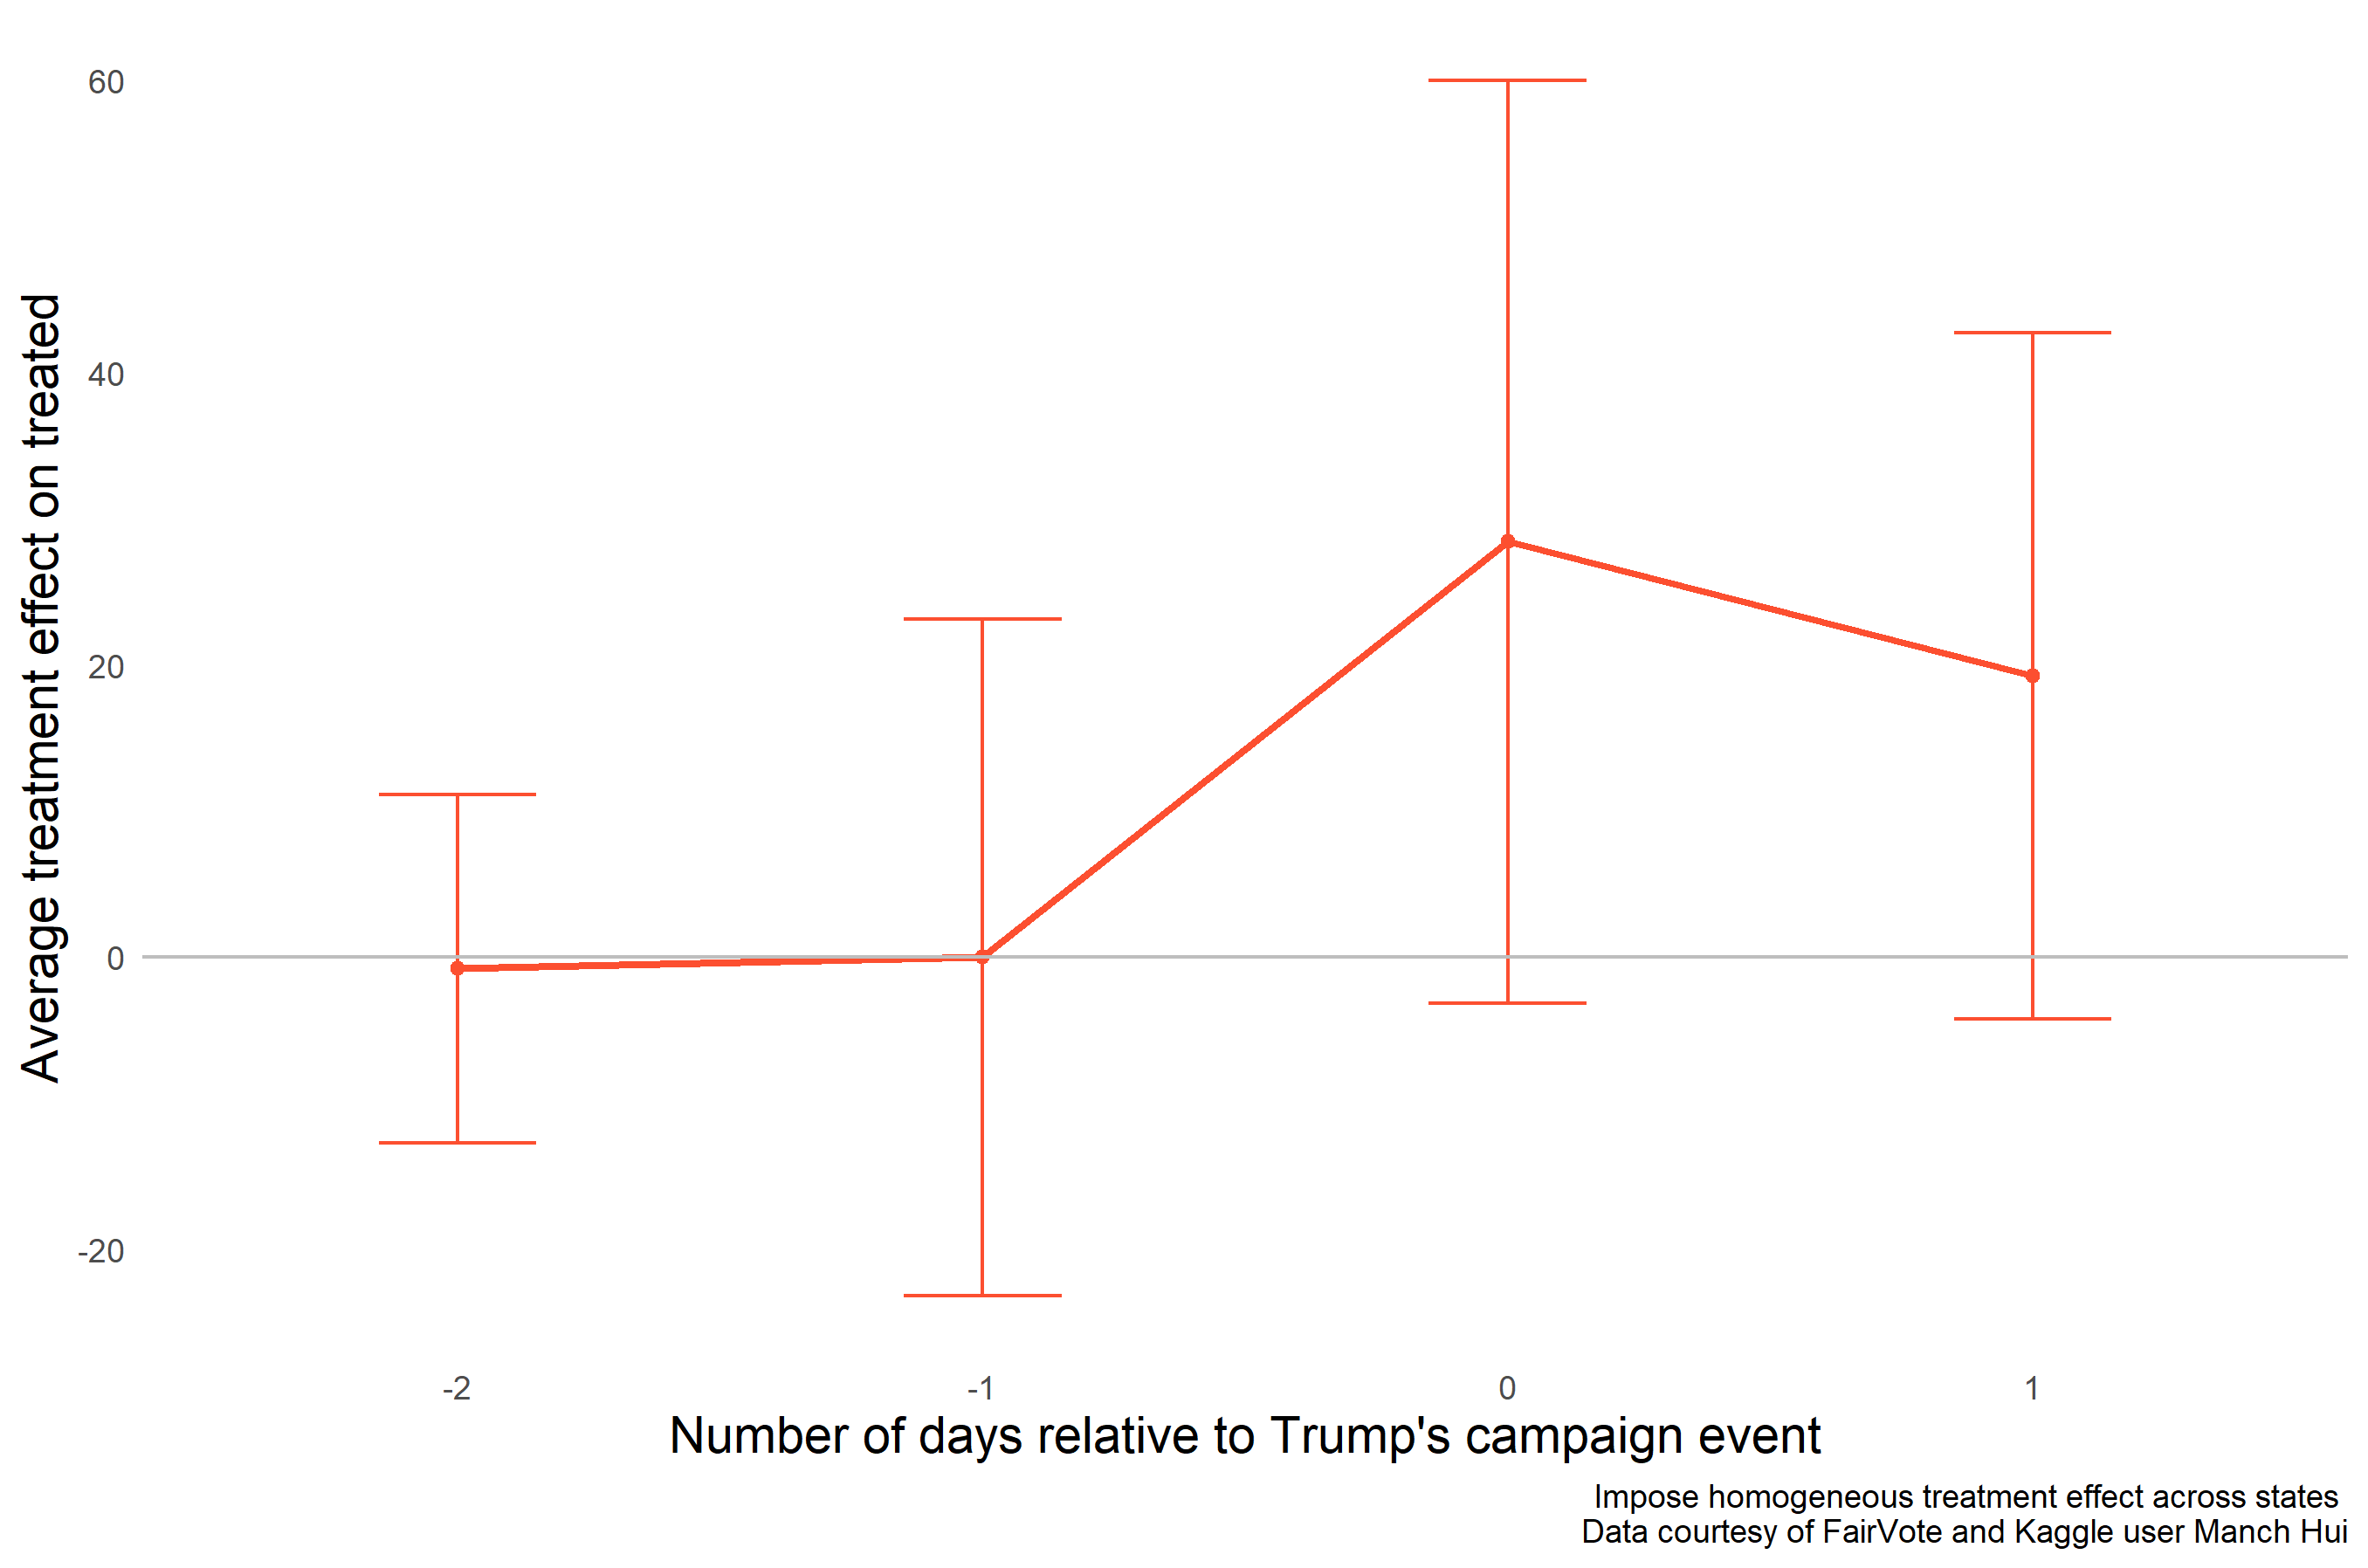
\includegraphics[width = 0.8 \textwidth]{C:/Users/Zhuxl/Box/projects/ra_code_sample/election_tweets/output/figures/event_study_reg_plot_trump.png}
		\caption{Average treatment effect over event time for Trump's twitter presence (impose homogeneous treatment effect across states)} \label{fig:2}
	\end{center}
\end{figure}
\end{document}
